
%% bare_jrnl.tex
%% V1.3
%% 2007/01/11
%% by Michael Shell
%% see http://www.michaelshell.org/
%% for current contact information.
%%
%% This is a skeleton file demonstrating the use of IEEEtran.cls
%% (requires IEEEtran.cls version 1.7 or later) with an IEEE journal paper.
%%
%% Support sites:
%% http://www.michaelshell.org/tex/ieeetran/
%% http://www.ctan.org/tex-archive/macros/latex/contrib/IEEEtran/
%% and
%% http://www.ieee.org/



% *** Authors should verify (and, if needed, correct) their LaTeX system  ***
% *** with the testflow diagnostic prior to trusting their LaTeX platform ***
% *** with production work. IEEE's font choices can trigger bugs that do  ***
% *** not appear when using other class files.                            ***
% The testflow support page is at:
% http://www.michaelshell.org/tex/testflow/


%%*************************************************************************
%% Legal Notice:
%% This code is offered as-is without any warranty either expressed or
%% implied; without even the implied warranty of MERCHANTABILITY or
%% FITNESS FOR A PARTICULAR PURPOSE! 
%% User assumes all risk.
%% In no event shall IEEE or any contributor to this code be liable for
%% any damages or losses, including, but not limited to, incidental,
%% consequential, or any other damages, resulting from the use or misuse
%% of any information contained here.
%%
%% All comments are the opinions of their respective authors and are not
%% necessarily endorsed by the IEEE.
%%
%% This work is distributed under the LaTeX Project Public License (LPPL)
%% ( http://www.latex-project.org/ ) version 1.3, and may be freely used,
%% distributed and modified. A copy of the LPPL, version 1.3, is included
%% in the base LaTeX documentation of all distributions of LaTeX released
%% 2003/12/01 or later.
%% Retain all contribution notices and credits.
%% ** Modified files should be clearly indicated as such, including  **
%% ** renaming them and changing author support contact information. **
%%
%% File list of work: IEEEtran.cls, IEEEtran_HOWTO.pdf, bare_adv.tex,
%%                    bare_conf.tex, bare_jrnl.tex, bare_jrnl_compsoc.tex
%%*************************************************************************

% Note that the a4paper option is mainly intended so that authors in
% countries using A4 can easily print to A4 and see how their papers will
% look in print - the typesetting of the document will not typically be
% affected with changes in paper size (but the bottom and side margins will).
% Use the testflow package mentioned above to verify correct handling of
% both paper sizes by the user's LaTeX system.
%
% Also note that the "draftcls" or "draftclsnofoot", not "draft", option
% should be used if it is desired that the figures are to be displayed in
% draft mode.
%
\documentclass[journal]{IEEEtran}

\usepackage{blindtext}
\usepackage[style=ieee,backend=biber]{biblatex}
\usepackage[final]{microtype}
\usepackage{csquotes}
\usepackage[english]{babel} 
\usepackage{array}

\usepackage{hyperref}
\addbibresource{references.bib}

\usepackage{caption}
\usepackage{graphicx}
\graphicspath{ {images/} }

\newcolumntype{L}[1]{>{\raggedright\let\newline\\\arraybackslash\hspace{0pt}}m{#1}}
\providecommand*{\opt}[1]{\texttt{#1}}
\providecommand*{\pkg}[1]{\textsf{#1}}


\begin{document}
%
% paper title
% can use linebreaks \\ within to get better formatting as desired
\title{Probabilistic Policy Violation Detection with IPFWD}

\author{Philip Nelson and Austin Voecks% <-this % stops a space
Western Washington University
\thanks{Supported in part by Dell EMC Isilon through grant and hardware}}


% The paper headers
\markboth{March~2017}%
{Shell \MakeLowercase{\textit{et al.}}: Bare Demo of IEEEtran.cls for Journals}
% The only time the second header will appear is for the odd numbered pages
% after the title page when using the twoside option.
% 
% *** Note that you probably will NOT want to include the author's ***
% *** name in the headers of peer review papers.                   ***
% You can use \ifCLASSOPTIONpeerreview for conditional compilation here if
% you desire.

% make the title area
\maketitle


\begin{abstract}
%\boldmath
When using a firewall system like IPFW to detect threats, we can end up doing a
lot of packet processing. This can negatively impact performance-sensitive
systems such as storage nodes in data centers. This paper describes a
practical solution to this problem using a load-weighted probabilistic
mechanism that allows a trade-off between perfect visibility of incoming
packets and reduced impact to system load.  

\end{abstract}


% Note that keywords are not normally used for peerreview papers.
\begin{IEEEkeywords}
FreeBSD, IPFW, firewalls, performance.
\end{IEEEkeywords}


% For peer review papers, you can put extra information on the cover
% page as needed:
% \ifCLASSOPTIONpeerreview
% \begin{center} \bfseries EDICS Category: 3-BBND \end{center}
% \fi
%
% For peerreview papers, this IEEEtran command inserts a page break and
% creates the second title. It will be ignored for other modes.
\IEEEpeerreviewmaketitle


\section{Introduction}

  Firewalls shield networks and hosts from malicious traffic by blocking
  network packets that do not match any of the rules defined in a security
  policy. 
  In high performance and network throughput environments, extensive packet
  processing by firewalls can limit the system's ability to utilize the full
  capacity of network links. This problem is typically addressed by restricting
  the number and complexity of firewall rules, disabling the firewall entirely,
  or sacrificing the additional throughput so all the packet processing can be
  completed.
  
%  The default action for white-list firewalls is to block all traffic,
%  additional rules describe exceptions. Blacklist firewalls are the opposite,
%  by default they accept all traffic and additional rules describe packet types
%  that are not allowed. Since predicting and blacklisting all possible attacks
%  is not possible in practice, white-list firewall rule sets are the accepted
%  standard and the focus of this paper. Without a security policy,
%  administrators cannot know what to allow and disallow when constructing
%  firewall rules.

    % Packet sampling
    Other papers \cite{exploitingpacketsampling, analysisnetflow,
    monitoringpacketsampling} on packet sampling have been focused on detecting
    and classifying threats, not performance enhancement. However, their
    approaches to packet sampling and the implications addressed provided the
    inspiration for the work done here. The BSD community has produced several in depth investigations into network
    and firewall performance \cite{ipfwvspf,optimizingfreebsd}. Their work
    informed the tests run here.


\section{IPFW \& IPFWD}

  IPFWD is a daemon for FreeBSD that updates an early rule in IPFW (the IP
  Firewall) that has a chance to accept any packet. The probability of early
  acceptance is updated over time and dependent on the current system load. In
  high performance systems this can result in an increase in network
  throughput.

  This approach is based on the premise that firewall performance can be
  improved by reducing the number of rules applied to each packet. Supposing a
  white-list policy, a firewall must apply every rule to a packet before
  it's denied.  With IPFWD, the system has a chance to accept any packet early
  and skip any further computation. Test results show this reduces the 
  resources required to handle the same amount of traffic in some systems.

  This is a shift in mindset from typical firewalls \cite{networksecurity}.
  Instead of enforcing every part of the security policy all the time, IPFWD
  enforces the policy some of the time provides additional information so the
  missed violations can be inferred. For this cost, you gain increased firewall
  performance and network throughput in resource bound systems. IPFWD works
  under the assumption that it's acceptable to allow a percentage of policy
  violations given that network traffic patterns are often repeated and the
  goal is detection, not immediate prevention. Administrative action may be
  taken later when resource requirements are lower.

  As an example, under heavy load IPFWD may immediately accept 40\% of packets.
  Some of those packets may have been malicious. Supposing a port scan was
  initiated during this time and rules exist to block it, at least 60\% of the
  port scan would still be rejected and logged. Since the early acceptance
  probability will fluctuate over time, IPFWD provides information in the IPFW
  logs to show the chance undetected violations occurred for each detected
  violation. IPFWD allows administrators to keep extensive rule sets that fully
  implement their security policy. Instead of having to simplify rule sets to
  increase performance, IPFWD balances policy enforcement and performance
  automatically. Under normal or light load, IPFWD will enforce the entire
  security policy 100\% of the time.

  % Why was this firewall chosen?
  \subsection{Choice of IPFW}

    IPFW is a stateful firewall written for FreeBSD which supports both IPv4
    and IPv6. It is comprised of several components: a kernel firewall filter
    rule processor and its integrated packet accounting facility, a logging
    facility, NAT, the dummynet traffic shaper, a forward facility, a bridge
    facility, and an ipstealth facility \cite{freebsdhandbook}.

    IPFW was chosen for its close integration with the FreeBSD operating
    system, kernel packet filter, and performance. Performance is dependent on
    system parameters and circumstances, but IPFW outperforms the other main
    firewall option for FreeBSD, PF, in stateful packet filtering
    \cite{ipfwvspf}. Stateful rules are more powerful and flexible than
    stateless rules, where no session information is maintained
    \cite{networksecurity}.  Additionally, the capabilities of IPFW extend
    beyond packet filtering into source based routing, traffic shaping and
    more. It's for these reasons that IFPW was chosen over PF.

    % First match wins rule system and probabilistic matching
    Firewall rules are treated by IPFW in a first-match-wins fashion. IPFW also
    contains built-in functionality and rule syntax for probabilistic packet
    matching. From the documentation, this feature was intended for load
    balancing and other traffic shaping tasks. It's the core of IPFWD's
    operation. 


\section{IPFWD}

  % What does it do?
  IPFWD increases firewall performance by reducing the average amount of work
  it takes to process a packet. Depending on the current system load, IPFWD
  increases or decreases the chance the IPFW will accept a given packet early.
  It does this by adding and maintaining an early rule in the IPFW rule set of
  the following form: 
  \begin{center}
      \verb|prob 0.000 allow ip from any to any|
  \end{center}
  which allows any IP packet, incoming or outgoing with a chance equal to the
  probability given.

  % How does it work?
  % - Probabilistic packet matching
  IPFWDs behavior is based on the assumption that the majority of network
  traffic is valid, malicious events are rare \cite{networktrafficanalysis},
  and it's sufficient to be notified of security policy violations instead of
  always stopping them. These assumptions will not hold in all environments,
  but we can leverage them for performance gains when they do.

  Since IPFW uses a first-match-wins rule system, this early rule will be
  encountered before the majority of the other rules in the rule set.  The
  probability given in this rule determines the chance that IPFWD skips
  processing all further rules, supposing that there has not been a match
  already.  

  This is especially valuable for a white-list firewall rule set dealing with
  large amounts of rejected traffic; normally each rejected packet has all
  rules applied to it in order to find a match. When no matches are
  encountered, the default rule is employed and the packet is rejected. 

  In a typical data center internal network, the vast majority of traffic is
  valid and going to be accepted by the firewalls rule set. However, these rule
  sets are often complex and take increasing time to match packets depending on
  the number of rules. For a rule set of length $n$, we can expect a packet to
  encounter on average $\frac{n}{2}$ failed matches before matching the correct
  rule and being accepted.

  IPFWD improves the average number of failed matches before a successful match
  from

  \[
  \frac{n}{2}
  \]

  to

  \[
  \Big(k \cdot \mathsf{P}(\textit{EA})\Big) + 
  \Big(\frac{n}{2} \cdot \mathsf{P}(\neg{\textit{EA}})\Big) 
  \]

  where $k$, a small constant compared to $n$, is number of rules before the
  early acceptance rule and $\mathsf{P}(\textit{EA})$ is the probability that
  the early acceptance rule is matched.

  Simplifying in order notation, IPFWD reduces the number of failed matches before
  a successful match by a factor of

  \[
  \frac
      {\frac{n}{2}}
      {\frac{n}{2} \cdot \mathsf{P}(\neg{\textit{EA}})} 
  = \frac{1}{\mathsf{P}(\neg{\textit{EA})}}.
  \]

  % - Log extension
  While this method increases the speed the system processes packets, it
  creates a chance that packets that would have normally been rejected will get
  through the firewall.

  In order to provide visibility into this process, IPFWD writes its own logs
  to include information about the early acceptance probability. From this
  information, administrators can extrapolate the probability that additional
  invalid packets made it through the firewall for each that is detected. This
  is discussed further in \ref{securityimplications}.

  % When should this system be used?
  \subsection{Application}

    IPFWD is not intended to be used on all types of systems. It's application
    instead most directly benefits the following types of systems:

    \begin{enumerate}
      \item \textbf{High Network Performance}

        The gains provided by IPFWD are only apparent in systems where network
        throughput is matched by or out performs CPU speed. Systems that can
        already easily handle fully processing each packet will not benefit by
        reducing processing time. Given modern CPU clock speeds, systems with
        network cards slower than 1 Gb/sec will likely not benefit from IPFWD.

      \item \textbf{Complex Firewall Requirements}

        IPFWD works by reducing the average number of rules that fail to match
        before a packet is finished being processed. Very simple rule sets will
        gain little from reducing the number of rules applied to each packet.

      \item \textbf{Detection Based Security Policy}

        By using IPFWD, administrators sacrifice the assurance that every
        invalid packet will be rejected.  However, they are still provided
        information as to whether some invalid packets were rejected, and that
        information can be used to infer the existence of additional invalid
        packets. Environments that cannot allow this relaxation in security
        policy enforcement will no benefit from IPFWD.

    \end{enumerate}


\section{Security Implications} \label{securityimplications}

  % Talk about security policy enforcement
  Security policies define what is and is not allowed in an organization. At
  the network and host level, this is implemented in part by a firewall rule
  set. A policy violation on an internal network is more serious than an
  external network. Internet facing hosts can expect to be scanned, experience
  network anomalies, and be attacked by third party agents more often than
  internal hosts. 

  However, when these events do occur on an internal network, there is a strong
  possibility something else is wrong. Unexpected network activity on a fully
  controlled internal network indicates compromise or misconfiguration, both of
  which are serious problems. The usage of IPFWD is predicated on the
  assumption that it's sufficient to be notified of these events so further
  action can be taken later.

  % What does it mean for security if you're ignoring some of the packet?
  Allowing some percentage of network packets through the firewall without
  inspection does mean that attacks that would have normally been blocked could
  succeed. The following factors help to account for this risk:

  \begin{enumerate}

    % Bad things are often repeated
    \item \textbf{Repetition} 

      Malicious network activity such as malware beaconing and network
      reconnaissance, as well as general network errors are likely to be
      repeated over time \cite{beacondetection}. The longer the activity
      persists, the more likely it is to be detected by IPFW, even when IPFWD
      is allowing a high percentage of the network traffic through unchecked.

    \item \textbf{Disruption} 

      Though some malicious network activity may only consist of a single
      packet, others will require multiple packets. Since IPFW works on a
      per-packet basis, malicious network activity will experience
      approximately $(1 - m)\%$ packet loss where $m$ is IPFWDs probability of early
      acceptance. The exact effect this would have on malware or reconnaissance
      would depend, but generally will increase the chance of failure or
      invalid results.

  \end{enumerate}

  % How do you trust this system?

  % Talk about shift in mindset from "blocking attacks" to "detecting attacks"
  % - Why is this reasonable?
  % - Is this really different than traditional firewalls?

  % example application
  \subsection{Example Scenario} 

    Suppose each host in a data centers internal network is running IPFW and
    IPFWD on each host, average CPU usage is $75\%$, and have rule sets
    blocking common network attacks. One of the hosts has been compromised and
    begins conducting network reconnaissance by port scanning the other hosts
    on the network. 

    Firewall rules are in place to block host-to-host communication to $m\%$ of
    the ports being scanned. This means that $1 - m\%$ of the scan would be
    allowed regardless of IPFWDs action. This percentage represents valid
    host-to-host communication as determined by the security policy.

    IPFWD would allow $75\%$ of the policy violating port scan through to the
    host, and $75\%$ of the replies back to the compromised host. This results
    in $75\% * 75\% = 56.25\%$ of the port scan that should have been stopped
    succeeding.  However, the other $1 - 56.25 = 43.75\%$ of the port scan was
    blocked and logged, alerting system administrators to the presence of
    malicious network activity so further action can be taken.

  % describe difference between reply and no reply violations
  Thus, the chance of missing a security policy violation depends on the type
  of traffic. The following situations exist when both incoming and outgoing
  firewall rules are employed:

  \begin{enumerate}

    % only one chance to catch
    \item \textbf{Incoming or Outgoing + No Reply}

      Here, the firewall only has one chance to catch the policy violation.
      So, if the early acceptance probability is $m$, then $m\%$ of the policy
      violating packets will be allowed.

    % two chances to catch 
    \item \textbf{Incoming or Outgoing + Reply}

      Here, the firewall has two chances to catch the policy violation. So,
      if the early acceptance probability is $m$, then $m'\%$ of the policy
      violating packets will be allowed where $m' = m * m$.

  \end{enumerate}


% Explain different systems and tests
\section{Benchmarking Performance}

  We benchmarked the performance of IPFW in relation to CPU usage and network
  throughput. The goal was to determine if IPFWD reduces the average time IPFW
  takes to process packets. Tests were run on three platforms and four
  different network cards, referred to as four different systems. The most
  important parameters to these tests are CPU, NIC, and ENV. Descriptions of
  each system are given in the tables below:\\

  % Isilon 40G
  \begin{tabular}{ | l | L{19em} | } 
    \hline
    \multicolumn{2}{|c|}{Isilon OneFS 40Gb System} \\
    \hline
    \hline
    OS  &  FreeBSD 11 Release \\
    CPU &  8 x64 Intel\textsuperscript{\textregistered}\ Xeon\textsuperscript{\textregistered}\ CPU @ 2.20GHz \\
    MEM &  64Gb \\
    NIC &  Ethernet 40Gbase-T \\ 
    ENV &  Physical \\ 
    \hline
  \end{tabular}\\\\

  % Isilon 10G
  \begin{tabular}{ | l | L{19em} | } 
    \hline
    \multicolumn{2}{|c|}{Isilon OneFS 10Gb System} \\
    \hline
    \hline
    OS  &  FreeBSD 11 Release \\
    CPU &  8 x64 Intel\textsuperscript{\textregistered}\ Xeon\textsuperscript{\textregistered}\ CPU @ 2.20GHz \\
    MEM &  64Gb RAM \\
    NIC &  Ethernet 10Gbase-T \\ 
    ENV &  Physical \\ 
    \hline
  \end{tabular} \\\\

  % WWU 1G
  \begin{tabular}{ | l | L{19em} | } 
    \hline
    \multicolumn{2}{|c|}{ WWU 1Gb System } \\
    \hline
    \hline
    OS  &  FreeBSD 11 Release \\
    CPU &  8 x64 Intel\textsuperscript{\textregistered}\ Core\texttrademark\ i7-2600 CPU @ 3.4GHz \\
    MEM &  16Gb \\
    NIC &  Ethernet 1000baseT \\ 
    ENV &  Physical \\ 
    \hline
  \end{tabular} \\\\

  % Virtualised 10G
  \begin{tabular}{ | l | L{19em} | } 
    \hline
    \multicolumn{2}{|c|}{ Virtualised 10G System } \\
    \hline
    \hline
    OS  &  FreeBSD 11 Release \\
    CPU &  1 x64 Intel\textsuperscript{\textregistered}\ Xeon\textsuperscript{\textregistered}\ CPU @ 1.80GHz \\
    MEM &  512Mb \\
    NIC &  Ethernet 10Gbase-T \\ 
    ENV &  Hypervisor \\ 
    \hline
  \end{tabular} \\\\

  The systems were tested on x64 FreeBSD 11 Release, with varying CPU type, CPU
  speed, RAM and network cards. Isilon and WWU systems were both physical
  hardware, while the Virtualised system was in a hypervisor environment hosted
  by a third party service.

  Virtualisation made it more difficult to have the same confidence in the
  results as with the physical machines. Tests on the Virtualised system were
  repeated additional times to account for the variability of the underlying
  physical hardware and contention between virtual machines.

  The WWU and Virtualised tests were conducted on stock FreeBSD 11 without
  additional network performance configuration applied. The Isilon systems
  contained additional network performance tuning and demonstrates the
  additional gains IPFWD can provide with careful FreeBSD 11 kernel
  configuration.

  \subsection{Netperf}

    % Explain tools
    Multiple network performance tools were explored but the final results were
    compiled using Netperf. Netperf generates network traffic between client
    and server instances and measures throughput, errors, and other network
    performance metrics. Netperf was chosen because it was readily available
    on all test platforms, provides built-in CPU utilization measurement, has a
    wide range of test types \cite{netperf}, and is used elsewhere in the BSD
    community for testing.

    % Explain tests
    The test type UDP\_STREAM was chosen over TCP\_STREAM for simplicity and to
    preserve CPU cycles for IPFW. Raw network throughput and CPU performance
    was the target metric, which can be difficult to assess with TCP
    \cite{netperf}.

    Netperf is single threaded, which allowed easier comparison of results
    between systems with different numbers of cores. Additionally, all tests
    were run while the system was idle to minimize contention over system
    resources. 

    % Experimental method
    All tests were conducted using the following setup:
    \begin{center}
    \begin{tabular}{ | L{10em} | L{10em} | } 
      \hline
      Machine 1 & Machine 2 \\
      \hline
      \hline
      \texttt{ipfw}        & \texttt{ipfw} \\
      \texttt{netserver}   & \texttt{ipfwd} \\
      \texttt{CPU monitor} & \texttt{netperf} \\
                           & \texttt{CPU monitor} \\
      \hline
    \end{tabular} \\
    \end{center}

  \subsection{CPU Measurement}

    CPU utilization measurement was the most difficult parameter to measure in
    these tests. There are many factors that can account for variability
    between tests and jitter in the results. The Netperf manual describes these
    challenges and the variety of techniques used on different systems to
    measure CPU usage \cite{netperf}.

    Netperf was run in single threaded mode, which explains why throughput was
    not closer to the maximum throughput for the NIC on each system. The
    FreeBSD network stack allows multithreaded packet processing by utilizing
    multiple queues meaning the kernel can spread the work done by IPFW over
    multiple cores \cite{freebsdhandbook}. Since we were indirectly testing the
    performance of IPFW through Netperf, there were two different CPU
    measurements to account for: kernel time and user time. Since IPFW runs in
    the kernel, its CPU time is classified as kernel time.

    Netperf was able to measure CPU utilization on the Virtualised and WWU
    systems, but didn't work on the Isilon systems. Instead, \textit{ps} was
    used. \texttt{ps} is a BSD utility that displays information about
    processes, including CPU utilization. We used \texttt{ps} to poll Netperf's
    CPU usage and averaged the output to get the results presented here. These
    tests are comparable since both measured user CPU utilization, not kernel
    CPU utilization. Thus, IPFWs CPU usage was measured indirectly through the
    CPU usage of netperf.


% Show results graphs, explain axises, etc
\section{Results}
  
  %  throughput & CPU
  \subsection{Throughput \& CPU}

    The graphs in figure \ref{fig:isiloncpu40}, \ref{fig:isiloncpu10},
    \ref{fig:wwucpu1}, and \ref{fig:virtualcpu10} show the interaction between
    CPU utilization and network throughput for each system with respect to
    IPFWDs early acceptance probability. The dashed lines are CPU utilization;
    solid is network throughput in Mb/second. A higher acceptance probability
    means a greater chance that a given packet was immediately accepted without
    further processing.

    The upward trend in throughput on the x-axis shows that as the early
    acceptance probability increases, so does throughput. The CPU usage shows
    that this additional throughput was gained without additional CPU
    utilization, meaning the system was spending fewer cycles to process each
    packet on average.

    The lack of any trend in the WWU 1G graph \ref{fig:wwucpu1} was expected
    and will be addressed in \ref{discussion}.
    
    \begin{figure}[h]
      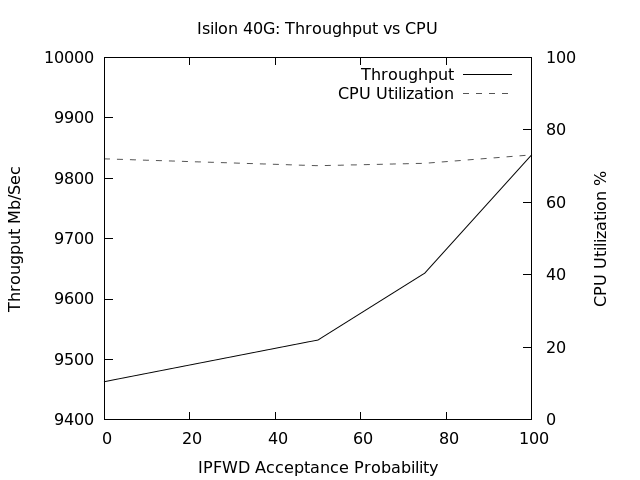
\includegraphics[width=0.45\textwidth]{cpu_isilon40}
      \caption{Throughput \& CPU for Isilon 40G system}
      \label{fig:isiloncpu40}
    \end{figure}
    \begin{figure}[h]
      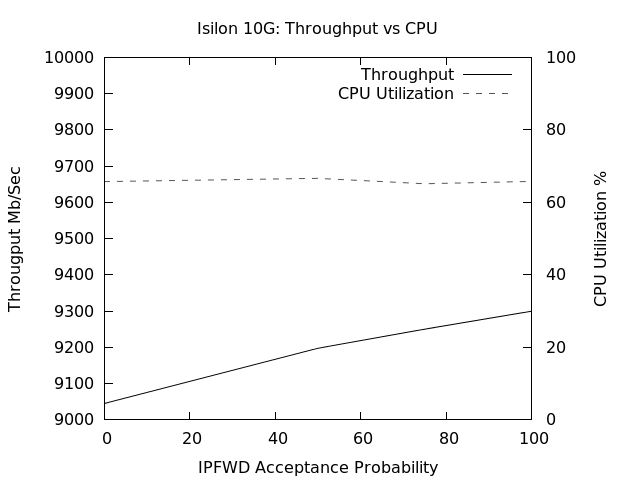
\includegraphics[width=0.45\textwidth]{cpu_isilon10}
      \caption{Throughput \& CPU for Isilon 10G system}
      \label{fig:isiloncpu10}
    \end{figure}
    \begin{figure}[h]
      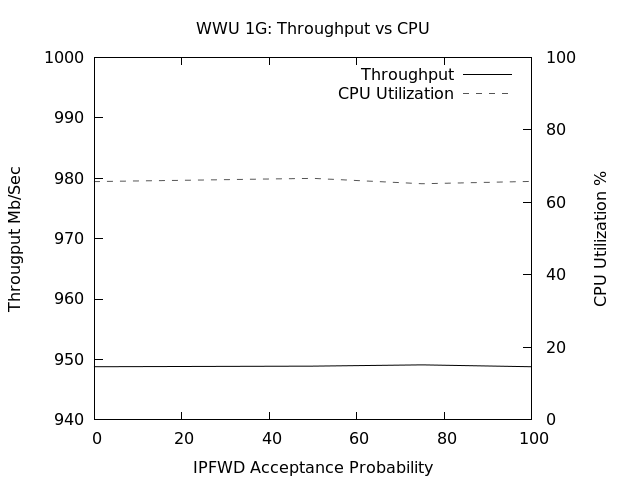
\includegraphics[width=0.45\textwidth]{cpu_wwu1}
      \caption{Throughput \& CPU for WWU 1G system}
      \label{fig:wwucpu1}
    \end{figure}
    \begin{figure}[h]
      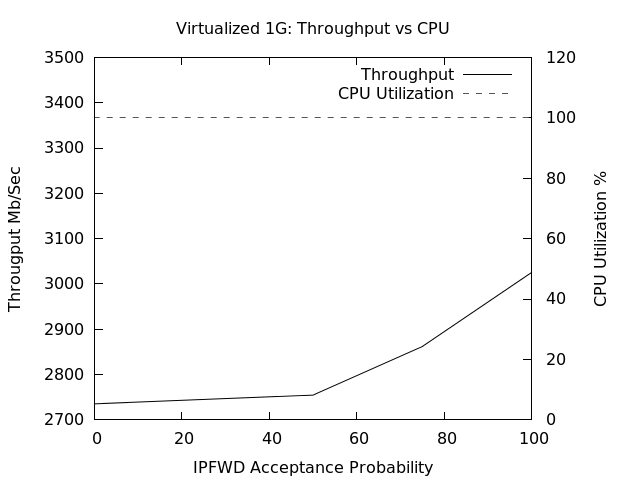
\includegraphics[width=0.45\textwidth]{cpu_virtual10}
      \caption{Throughput \& CPU for Virtualised 10G system}
      \label{fig:virtualcpu10}
    \end{figure}
    
  % throughput/CPU
  \subsection{Throughput / CPU}

    The graphs in figures \ref{fig:isilontoc40}, \ref{fig:isilontoc10},
    \ref{fig:wwutoc1}, and \ref{fig:virtualtoc10}  show network the ratio of
    throughput to CPU utilization for each system where $ratio(x) =
    throughput(x) / cpu(x)$. The data being presented here is the same as the
    previous graphs, merely shown differently. The upward trend over the x-axis
    shows that as the probability of early acceptance increases, the system is
    spending less CPU time to process packets on average.

    The dashed line shows the line of best fit for the throughput to CPU
    utilization ratio and shows the upward trend more clearly than the raw
    data.
    
    \begin{figure}[h]
      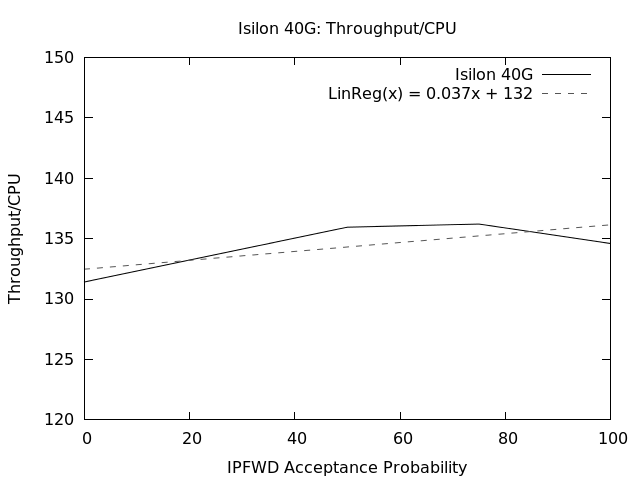
\includegraphics[width=0.45\textwidth]{toc_isilon40}
      \caption{Throughput/CPU for Isilon 40G system}
      \label{fig:isilontoc40}
    \end{figure}
    \begin{figure}[h]
      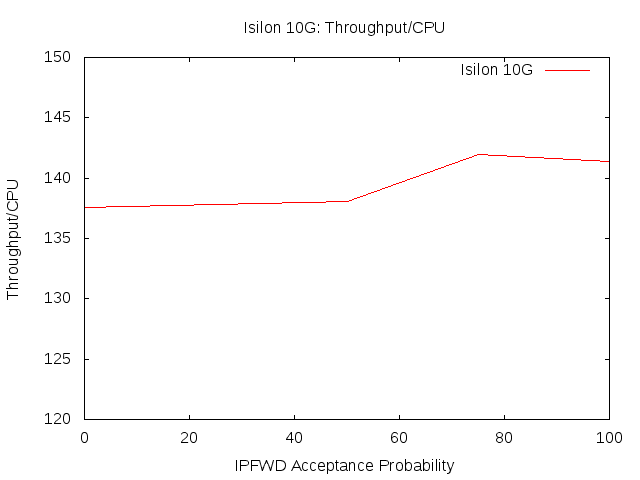
\includegraphics[width=0.45\textwidth]{toc_isilon10}
      \caption{Throughput/CPU for Isilon 10G system}
      \label{fig:isilontoc10}
    \end{figure}
    \begin{figure}[h]
      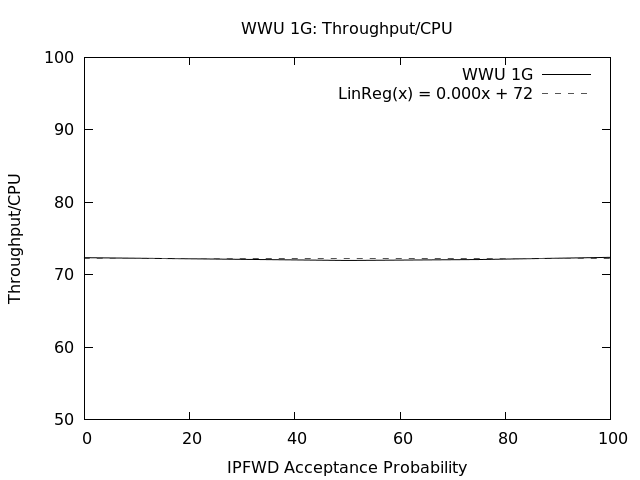
\includegraphics[width=0.45\textwidth]{toc_wwu1}
      \caption{Throughput/CPU for WWU 1G system}
      \label{fig:wwutoc1}
    \end{figure}
    \begin{figure}[h]
      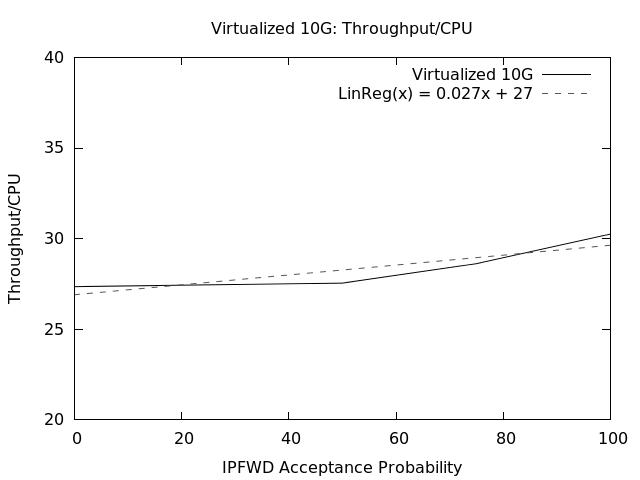
\includegraphics[width=0.45\textwidth]{toc_virtual10}
      \caption{Throughput/CPU for Virtualised 10G system}
      \label{fig:virtualtoc10}
    \end{figure}


  % Difference in results between CPU and throughput bound systems
  \section{Discussion} \label{discussion}

    All the systems tested can be broadly categorized into two groups: CPU
    bound and NIC throughput bound. We can see that IPFWD affects performance
    positively but differently for both types. 

    In CPU bound systems, IPFWD reduces the number of cycles it takes to
    process each packet, allowing more packets to be processed in the same time
    and increasing throughput. This is shown most clearly in the Virtualised
    system tests, which have the weakest CPU but 10Gb Ethernet NICs. Regardless
    of test type, the receiving system is always at 100\% CPU utilization.
    However, as the probability to accept increases in IPFWD the throughput
    also increases.  This clearly shows that IPFWD decreases the CPU time
    required to process incoming traffic.

    In NIC throughput bound systems, reducing the number of CPU cycles to
    process packets will not increase throughput. However, IPFWD still reduces
    CPU load which allows more cycles to be dedicated to other system
    processes. This is more difficult to see in the test results, particularly
    since the CPU measurement tools are inherently imprecise and difficult to
    compare between systems. 
    
    % WWU 1G
    However, the WWU 1G tests provide an example of a NIC bound system. The
    lack of any performance gains in the WWU 1G tests provides an example of
    when IPFWD should not be used. In this system, the CPU and other system
    resources are more than sufficient to apply the entire IPFW rule set to
    each packet at wire-speed. Reducing the amount of CPU time it takes to
    process each packet does not provide any benefit.

    In summary, systems where the throughput of the NIC exceeds what the CPU
    can supply CPU utilization is high and throughput is lower than the NIC
    maximum (eg: the Virtualised system \ref{fig:virtualcpu10}). Conversely,
    when CPU availability exceeds NIC throughput, throughput is high and CPU
    utilization is low (eg: the WWU 1G system \ref{fig:wwucpu1}).

    Additionally, all tests were run with minimal IPFW rule sets in a range of
    30 to 60 rules depending on the environment and network card configuration.
    Larger production rule sets would benefit even further from IPFWD.



\section{Future Work}

  % Firewall rule reordering so we can "fail as early as possible"
  Ideally, a white-list firewalls rule set would be constructed so that the
  most commonly applied matches are reached sooner rather than later. IPFWD
  accomplishes this task by artificial early stopping. Firewall rule reordering
  could be another solution to this problem. Given logs of common network
  traffic for the system, statistical analysis could show which rules are
  matched more often than others. With this information, the rule set could be
  reordered so that the most commonly applied rules are earliest. A combination
  of redundancy checking and priority reordering could provide further
  performance gains as well.

  % creating baseline invalid packet % so we can extrapolate even when we don't
  % see any invalid packets 
  Further analysis could be done to packet samples in order to more accurately
  determine appropriate bounds on the early acceptance probability. Different
  systems and environments may require more or less stringent packet checking.
  Environments with very high confidence in network security might raise the
  lower bound of the acceptance rate to improve performance. Likewise, less
  confident environments may lower the upper bound to ensure an acceptable
  percentage of packets are always checked.

  % mutli threaded netperf tests
  The tests conducted here were restricted to one core; future work could
  explore the interaction of early acceptance on parallel firewall packet
  processing. Running additional, concurrent netperf tests would show how the
  system behaves when the links are fully saturated.

  % have detection of bad traffic reduce acceptance rate
  Future versions of IPFWD could benefit from additional modifiers to the early
  acceptance probability. For instance, the system could reduce the early
  acceptance probability whenever packets are dropped by the firewall, under
  the assumption that invalid traffic likely precedes more invalid traffic.


\section{Conclusion}
  % What performance benefit do we get?
  % What security cost is there?
  % Why is this useful?
  % Why is this important?

  In performance sensitive computing environments, complex firewall rules
  combined with high network throughput can result in heavy CPU load, limiting
  system performance. IPFWD addresses this problem by providing a graceful
  trade off between packet visibility, total security policy enforcement and
  system performance.

  IPFWD reduces the average amount of work to process packets by adding an
  early rule to IPFW that has a chance to accept any packet. The security
  implications of this behavior have been addressed and the performance
  benefits provided have been demonstrated in a variety of systems.

  IPFWD can be directly applied to high network performance and resource
  conscious systems with complex firewall requirements to reduce CPU load and
  increase network throughput. This work also serves as a proof of concept for
  future probabilistic packet matching firewall implementations.


\appendices
\section{Additional Information}
  The source code for IPFWD, additional test results, and development cycle
  information may be found at \texttt{https://github.com/Gandalf-/ipfwd}.


\section*{Acknowledgment} 

The authors would like to thank Dell EMC Isilon for providing hardware, access
to clusters for testing, and funding for this research. The
resources and the advice on FreeBSD network capabilities/network performance
testing were invaluable. A portion of this work was done during a summer
internship at Dell EMC Isilon.


% Can use something like this to put references on a page
% by themselves when using endfloat and the captionsoff option.
\ifCLASSOPTIONcaptionsoff
  \newpage
\fi

% trigger a \newpage just before the given reference
% number - used to balance the columns on the last page
% adjust value as needed - may need to be readjusted if
% the document is modified later
%\IEEEtriggeratref{8}
% The "triggered" command can be changed if desired:
%\IEEEtriggercmd{\enlargethispage{-5in}}

% references section
\printbibliography

% that's all folks
\end{document}
